\subsection{Package com.sirius.sequenziatore.server.presenter}
\begin{figure}[H] \centering 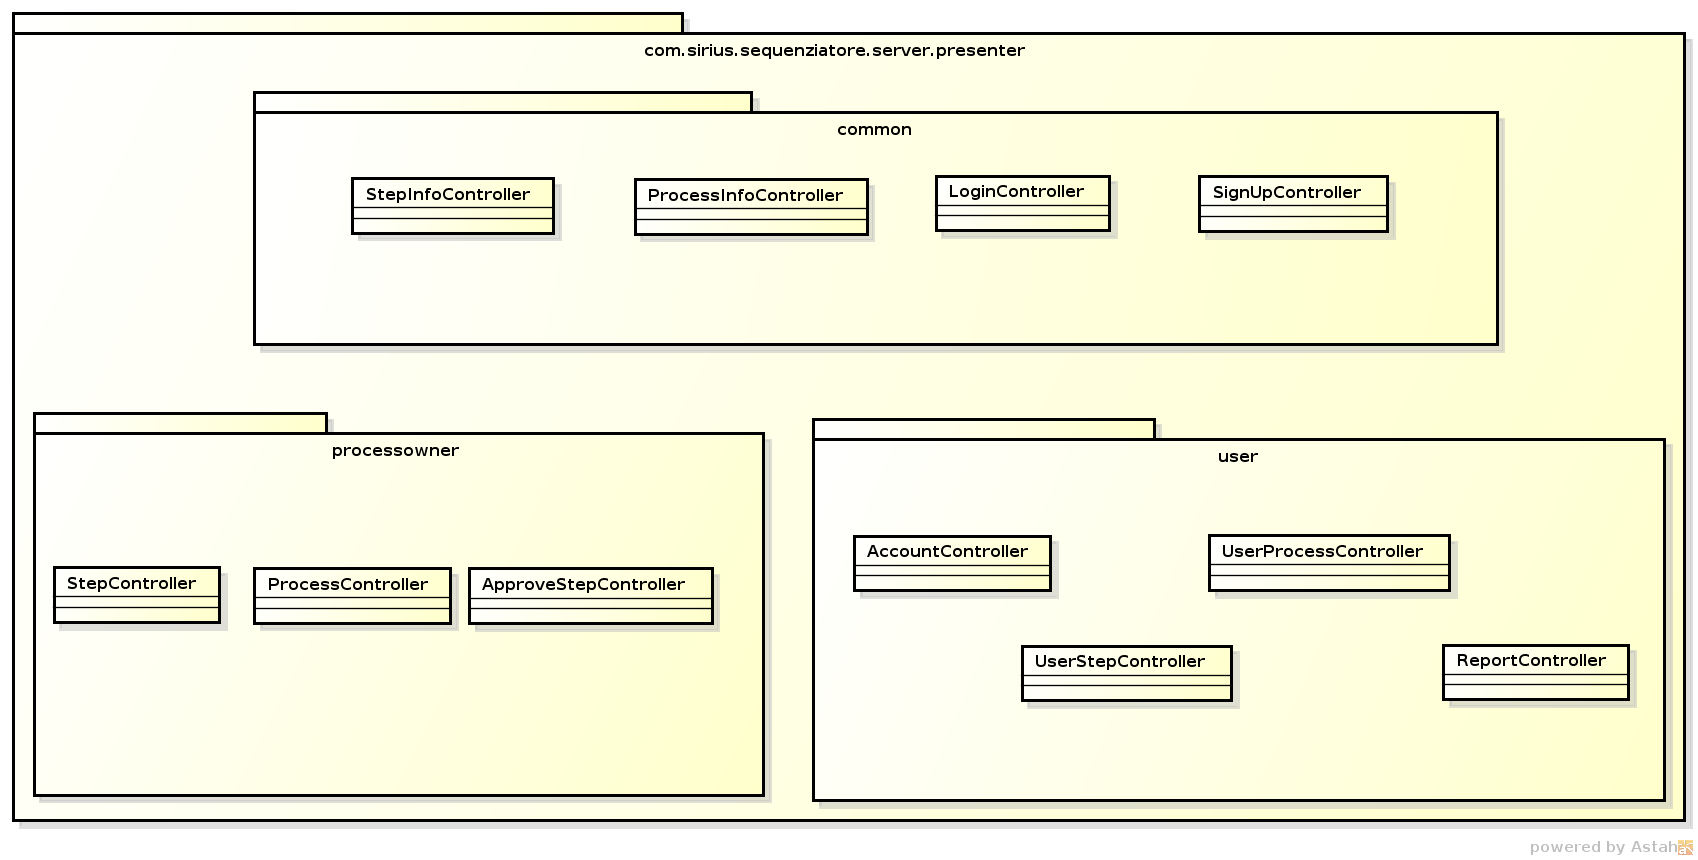
\includegraphics[width=%
\textwidth]
{./pack/ClassiServerSoloPresenter.png} \caption{Diagramma presenter server}
\end{figure}
\subsubsection{Package com.sirius.sequenziatore.server.presenter.common}
Questo \textit{package} contiene le classi che effettuano operazioni generali oppure comuni tra \textit{Process Owner} e Utenti.
\paragraph{LoginController}
	\begin{itemize}
		\item \textbf{Nome:} \texttt{LoginController};
		\item \textbf{Package:} com.sirius.sequenziatore.server.presenter.common
		\item \textbf{Descrizione:} Classe che permette la gestione della login di un utilizzatore del sistema, controllando che i dati inseriti riferiscano a un utente correttamente iscritto al sistema, ponendo attenzione se esso sia un \textit{process owner} o un utente normale;
		\item \textbf{Relazione con altre componenti:} la classe invoca i metodi della classe:
		\item \textbf{Relazione con altre componenti:} la classe invoca i metodi delle classi:
		\begin{itemize}
			\item com.sirius.sequenziatore.server.model.IDataAccessObject;
			\item com.sirius.sequenziatore.server.model.ITransferObject
		\end{itemize}
	\end{itemize}
	
\paragraph{SignUpConroller}
	\begin{itemize}
		\item \textbf{Nome:} \texttt{SignUpController};
		\item \textbf{Package:} com.sirius.sequenziatore.server.presenter.common
		\item \textbf{Descrizione:} Classe che permette la gestione della registrazione di un nuovo utente nel sistema, nonostante la correttezza dei dati inseriti venga controllata dalla parte client, per sicurezza verrà effettuato un nuovo controllo anche sulla parte server prima di inserire un utente nel sistema;
		\item \textbf{Relazione con altre componenti:} la classe invoca i metodi della classe:
		\item \textbf{Relazione con altre componenti:} la classe invoca i metodi delle classi:
		\begin{itemize}
			\item com.sirius.sequenziatore.server.model.IDataAccessObject;
			\item com.sirius.sequenziatore.server.model.ITransferObject
		\end{itemize}
	\end{itemize}
	
\paragraph{StepInfoController}
	\begin{itemize}
		\item \textbf{Nome:} \texttt{StepInfoController};
		\item \textbf{Package:} com.sirius.sequenziatore.server.presenter.common
		\item \textbf{Descrizione:} Classe che fornisce a chi lo richiede lo scheletro di un passo, quindi andrà a fornire i dati da inserire per tale passo e altre informazioni;
		\item \textbf{Relazione con altre componenti:} la classe invoca i metodi delle classi:
		\begin{itemize}
			\item com.sirius.sequenziatore.server.model.IDataAccessObject;
			\item com.sirius.sequenziatore.server.model.ITransferObject
		\end{itemize}
	\end{itemize}
\paragraph{ProcessInfoController}
	\begin{itemize}
		\item \textbf{Nome:} \texttt{ProcessInfoController};
		\item \textbf{Package:} com.sirius.sequenziatore.server.presenter.common
		\item \textbf{Descrizione:} Classe incaricata di fornire a chi lo richieda lo scheletro di un processo, come ad esempio numero di passi o condizioni per il suo completamento;
		\item \textbf{Relazione con altre componenti:} la classe invoca i metodi della classe:
		\item \textbf{Relazione con altre componenti:} la classe invoca i metodi delle classi:
		\begin{itemize}
			\item com.sirius.sequenziatore.server.model.IDataAccessObject;
			\item com.sirius.sequenziatore.server.model.ITransferObject
		\end{itemize}
	\end{itemize}

